\documentclass{article}

\usepackage{amsmath}
\usepackage{minted}
\usepackage{graphicx}
\usepackage{caption}
\usepackage{subcaption}

%Section style
\usepackage{etoolbox} %for configuration of sloppy
\usepackage{xcolor}


\definecolor{secnum}{RGB}{102,102,102}

\makeatletter
    \def\@seccntformat#1{\llap{\color{secnum}\csname the#1\endcsname\hskip 16pt}}
\makeatother
%end section style

\begin{document}

\section{I.2.1}

We are using the guassian function:
\begin{equation}
    f(x) = a * exp\left(-\frac{(x-b)^2}{2c^2}\right)
\end{equation}
Where:
\begin{align*}
    a &= \frac{1}{\sigma \sqrt{2\pi}}\\
    b &= \mu\\
    c &= \sigma 
\end{align*}
Giving us the full equation:
\begin{equation}
    f(x) = \frac{1}{\sigma \sqrt{2\pi}} * exp\left(-\frac{(x-\mu)^2}{2\sigma^2}\right)
\end{equation}
Using matlab we implemented (2) in the following code, giving us the figures \ref{fig:I1.1}

\begin{minted}{matlab}
    function
    end
\end{minted}

\begin{figure}[h!]
    \centering
    \begin{subfigure}[b]{0.5\textwidth}
        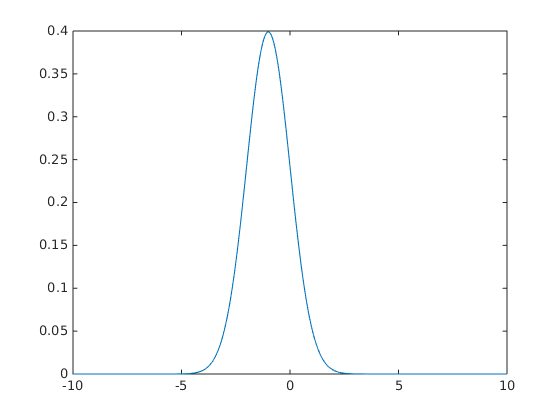
\includegraphics[width=\textwidth]{I211.png}
        \caption{$(\mu, \sigma) = (-1,1)$}
    \end{subfigure}%
    \begin{subfigure}[b]{0.5\textwidth}
        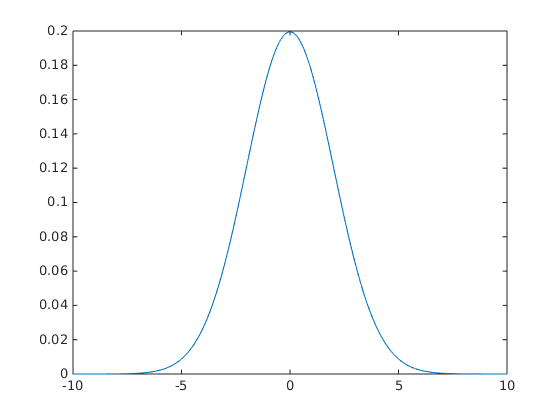
\includegraphics[width=\textwidth]{I212.png}
        \caption{$(\mu, \sigma) = (0,2)$}
    \end{subfigure}
    ~ %add desired spacing between images, e. g. ~, \quad, \qquad, \hfill etc.
    %(or a blank line to force the subfigure onto a new line)
    \begin{subfigure}[b]{0.5\textwidth}
        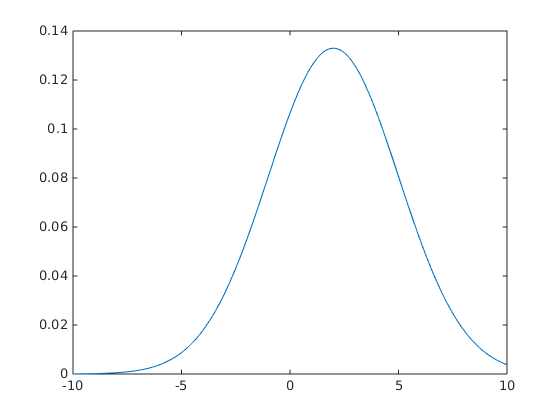
\includegraphics[width=\textwidth]{I213.png}
        \caption{$(\mu, \sigma) = (2,3)$}
    \end{subfigure}
    \caption{Gaussian distribution with varying parameters}
    \label{fig:I1.1}
\end{figure}




\end{document}
